\documentclass{beamer}
\usepackage{graphicx}  %import images
\usepackage{float} %control float positions
\usetheme[progressbar=frametitle]{metropolis}
\setbeamertemplate{frame numbering}[fraction]
\useoutertheme{metropolis}
\useinnertheme{metropolis}
\usefonttheme{metropolis}
\usecolortheme{spruce}
\setbeamercolor{background canvas}{bg=white}
\usepackage{multicol}

\setbeamercovered{transparent=	5}

\title{FDR Presentation}
\author{Jinxi Liu}
\begin{document}
\metroset{block=fill}
	
\begin{frame}
	
\titlepage
	
\end{frame}

\begin{frame}[t]{Slide Title}\vspace{10pt}
	\begin{enumerate}
		\begin{multicols}{2}
		\item item1
		\item item2
	\end{multicols}

	\end{enumerate}
	
	\begin{enumerate}[(A)]
		\item item A
		\item item B
	\end{enumerate}
	
	
\end{frame}

\begin{frame}[t]{Slide Title2}\vspace{10pt}
\begin{block}{Theorem}
	xxx...
\end{block}

\vspace{10pt}
xx \only<1>{\line(1,0){20}} 
   \only<2>{\textcolor{red}{answer1}}
   \only<3>{\textcolor{blue}{answer2}}
\, yy


\end{frame}

\begin{frame}{Slide Title3}\vspace{10pt}
 \begin{columns}[onlytextwidth]
 	
 	\column{0.33\textwidth}
 	 \only<1,2>{
 	 	Column A\\[10pt]
 	 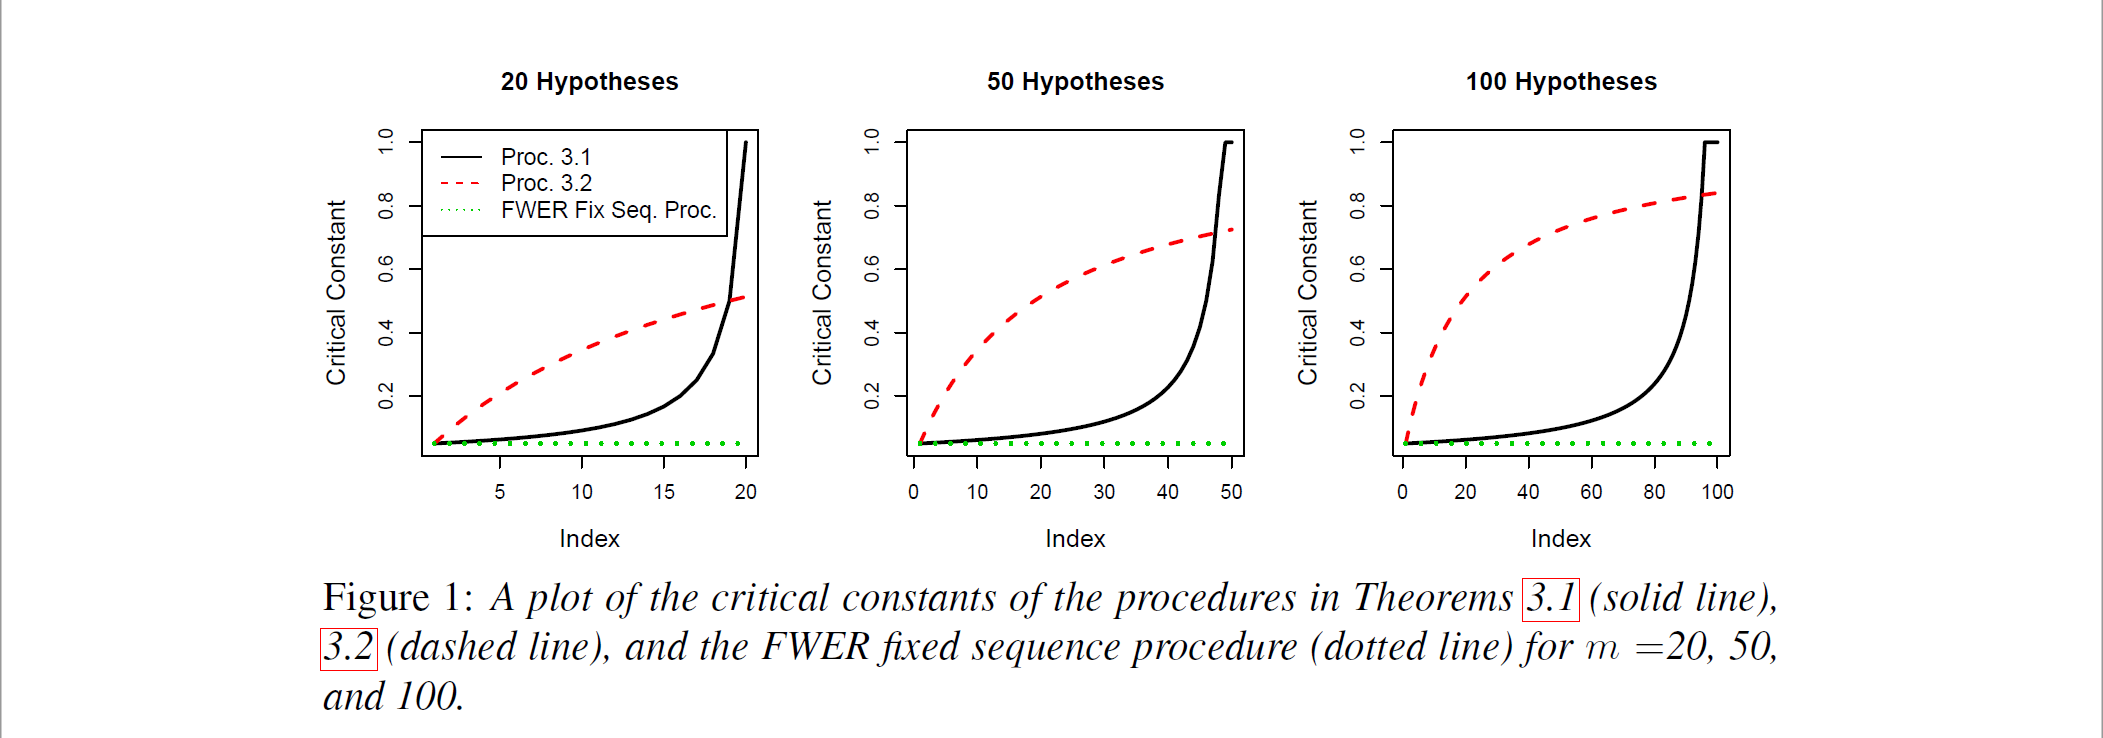
\includegraphics[scale=0.15]{test}
 	}
 	\column{0.33\textwidth}
 	\onslide<2>{                    % onslide = hide; only = erase
  	   Column B\\[10pt]
 	  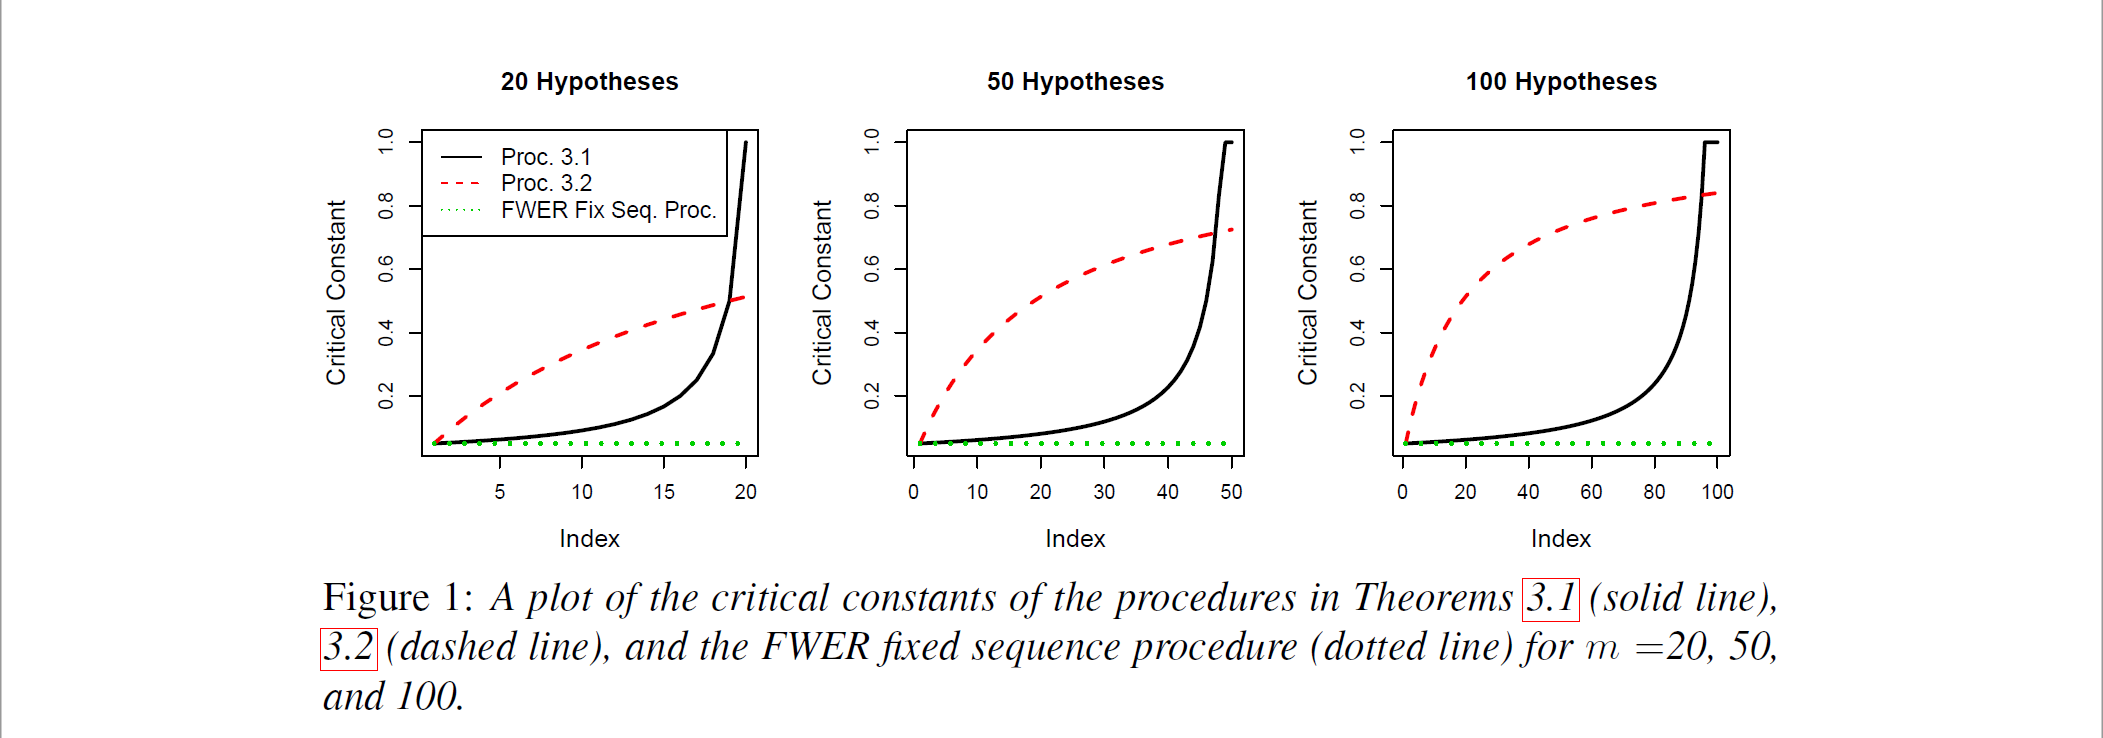
\includegraphics[scale=0.15]{test}
 	}
 	  \column{0.33\textwidth}
 	  \only<2,3>{
 	   Column C \\[10pt]
 	    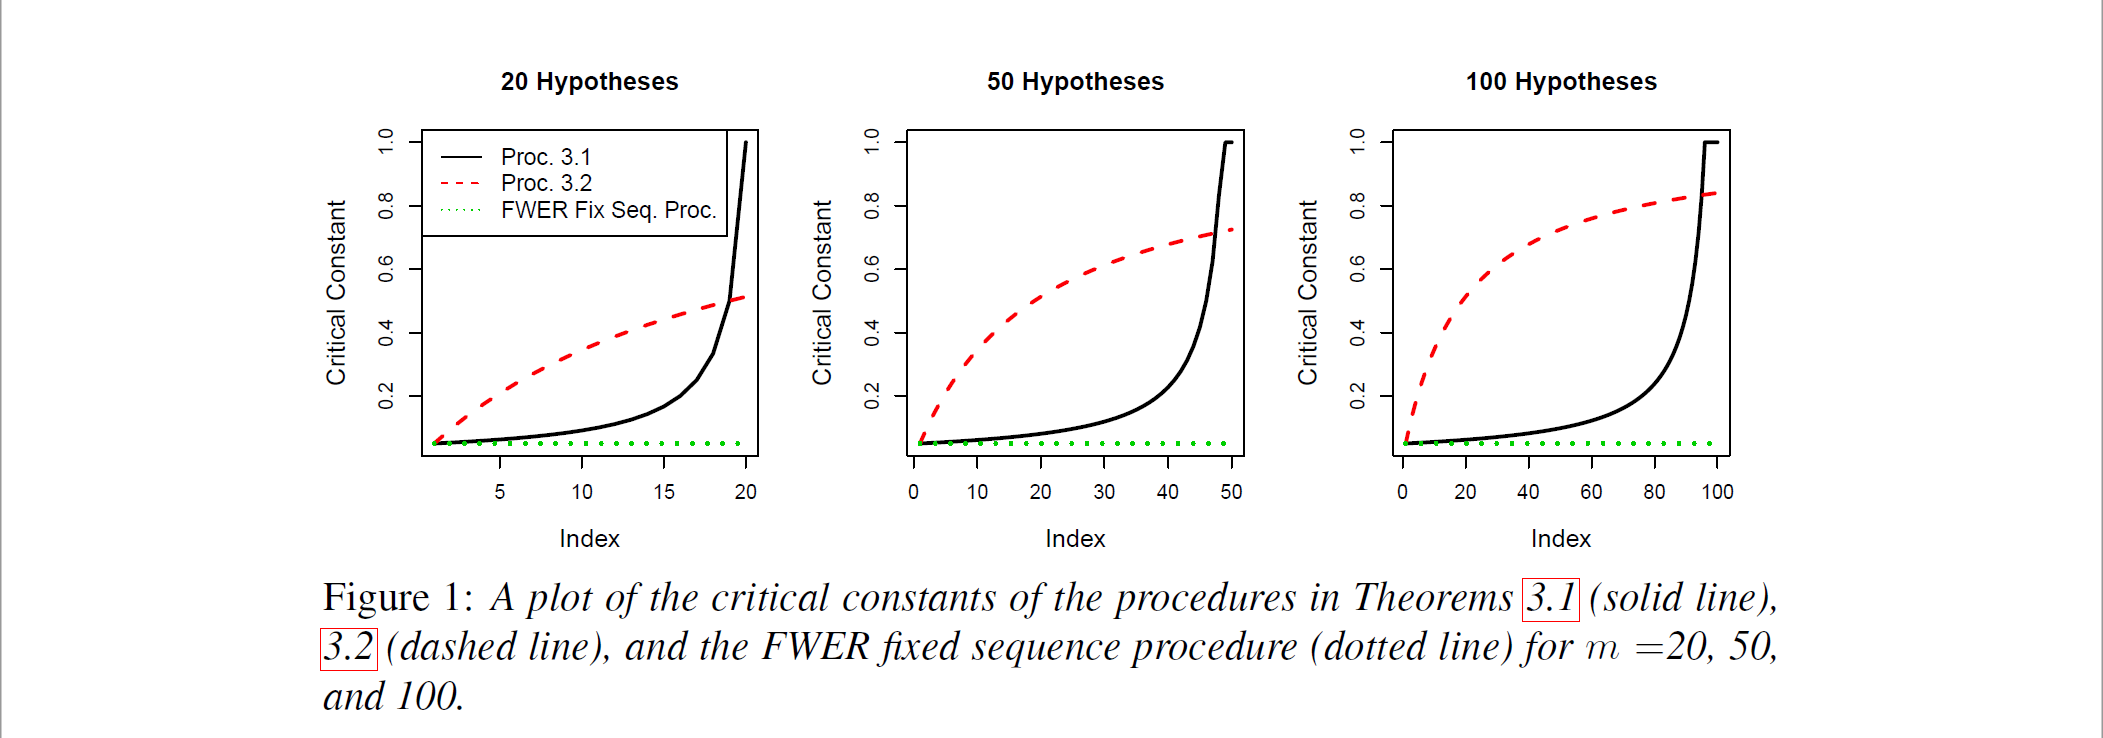
\includegraphics[scale=0.15]{test}
 	}
 \end{columns}
\end{frame}

\begin{frame}[standout]
\flushleft
Acknowledgement
\end{frame}

\end{document}